\begin{figure}[htpb]
	\centering\capstart{}
	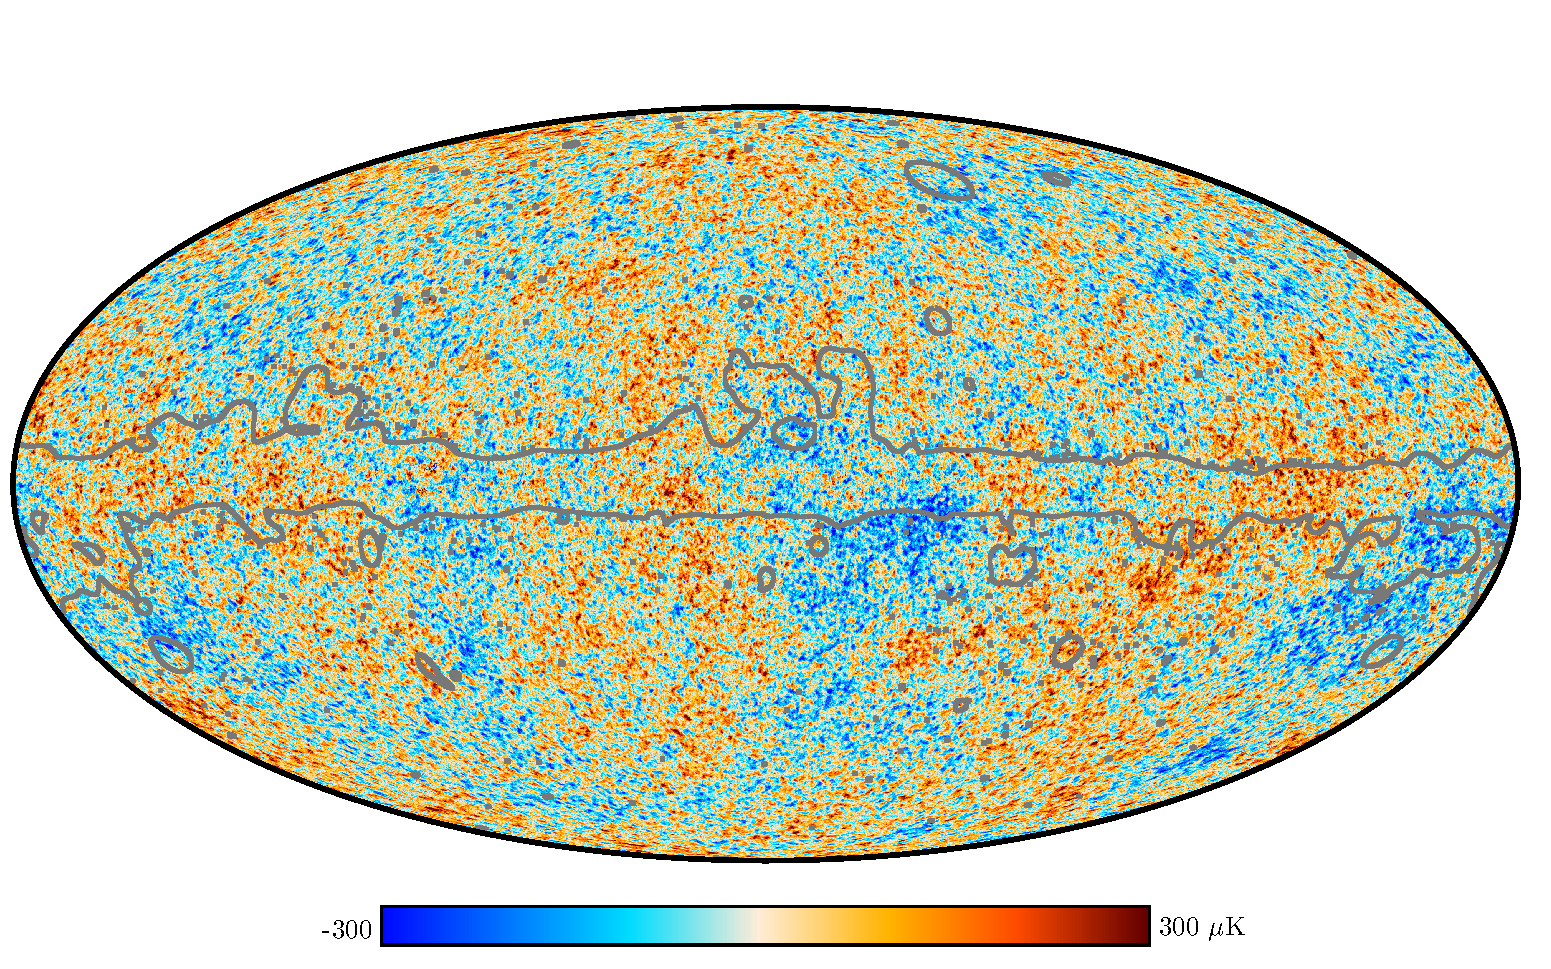
\includegraphics[width=\textwidth]{planck_2018_temp_mask.pdf}
	\caption[
		The 2018 Planck CMB map with the \texttt{Commander} mask
	]{
		The Planck \texttt{Commander} CMB temperature map used in low-\(\ell{}\) temperature likelihood analysis, smoothed to \(\SI{60}{\arcminute}\) FWHM resolution (courtesy of The Planck Collaboration 2018~\cite{Planck2020a}).
		The region in grey is the mask adopted for the likelihood analysis, which preserves \(\SI{86}{\percent}\) of the sky.
		Rather than developing methods to estimate a full-sky map, Slepian wavelets offer an alternative approach in which the wavelets are constructed in the region outside the mask.
	}\label{fig:chapter2_planck_masked}
\end{figure}
